\begin{titlepage}
    \newgeometry{top=1cm, width=21cm, bottom=1cm}
    \begin{center}
        \tikz[remember picture,overlay] \node[opacity=0.3,inner sep=0pt, anchor=east] at (current page.east){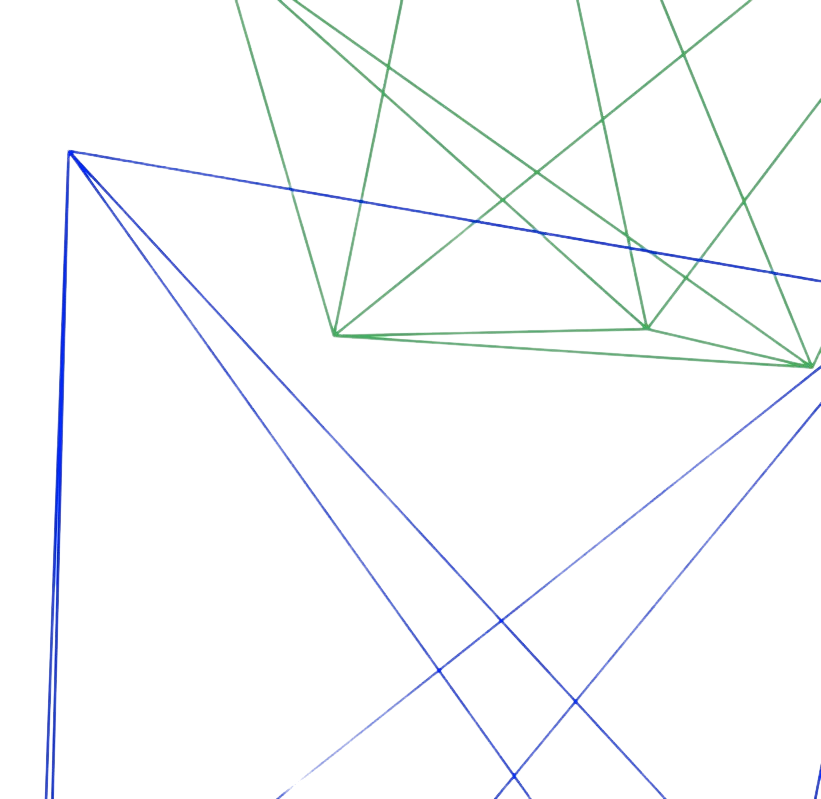
\includegraphics[width=0.5\paperwidth,height=\paperheight]{./logos/invert1.png}};
        \tikz[remember picture,overlay] \node[opacity=0.3,inner sep=0pt, anchor=south west] at (current page.south west){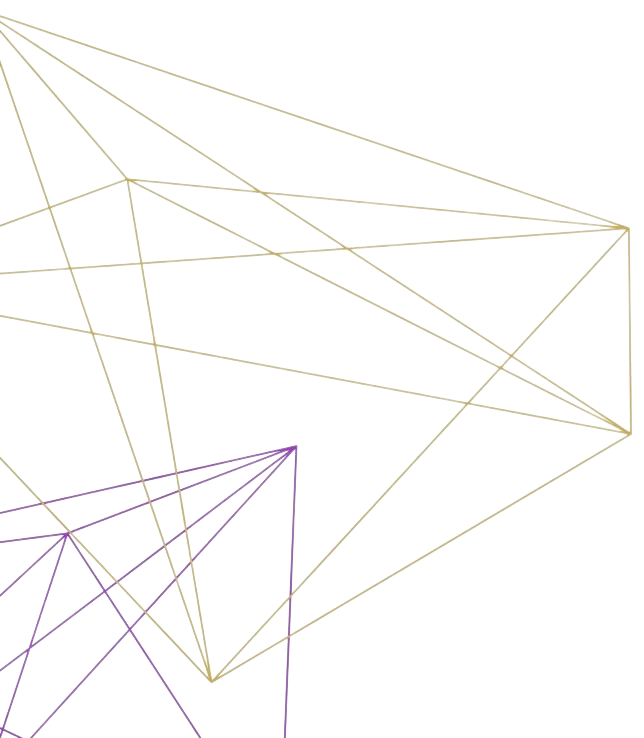
\includegraphics[width=0.5\paperwidth,height=0.5\paperheight]{./logos/invert2.png}};
        \tikz[remember picture,overlay] \node[opacity=0.3,inner sep=0pt, anchor=north west] at (current page.north west){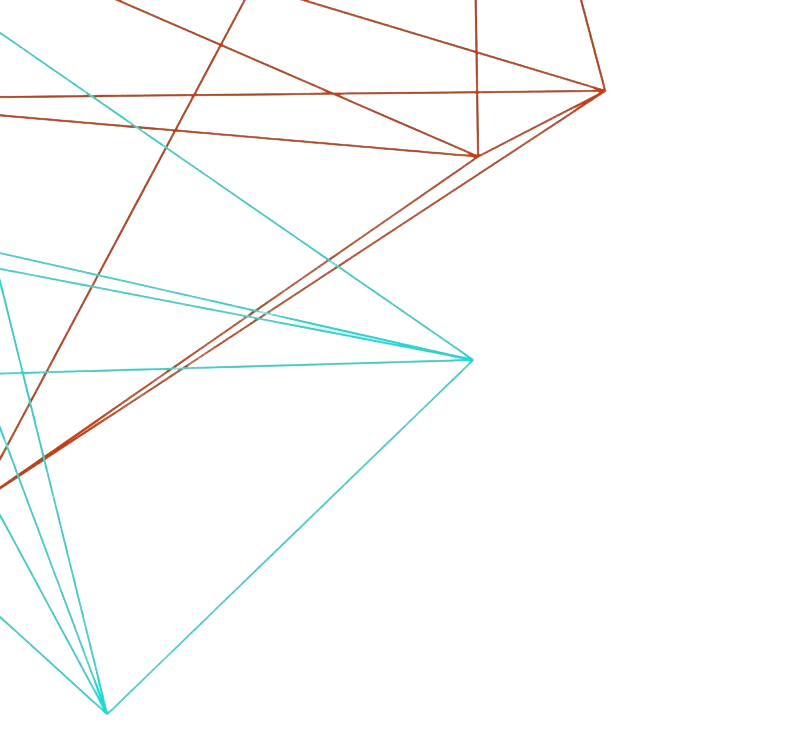
\includegraphics[width=0.5\paperwidth,height=0.5\paperheight]{./logos/invert3.png}};
    \end{center}


    \begin{tikzpicture}[remember picture,overlay,every node/.style={anchor=center}]
        \node (rectangle) at (page cs:0,0.4) [draw,thick, fill=white, minimum width=2cm,minimum height=2cm] {\HUGE\textbf{ DIFFERENTIAL EQUATIONS}};
    \end{tikzpicture}

    \begin{figure}[ht]
        
\includegraphics[height=1cm]{./logos/edx.png}
        \hspace{0.5cm}
        
\includegraphics[height=1cm]{./logos/Logo-W.jpg}
        \hspace{0.5cm}
        
\includegraphics[height=1cm]{./logos/OCW.png}
    \end{figure}

    \vspace{10cm}

    \begin{figure}[h]
        \centering
        
\includegraphics[width=0.5\textwidth]{./logos/Logo-old.png}
    \end{figure}
    \vspace{1cm}

\end{titlepage}
\newgeometry{width=18.625cm, bottom=2cm, top=2cm}

\tikz[remember picture, overlay] \node[opacity=0.3,inner sep=0pt, anchor=north east] at (current page.north east){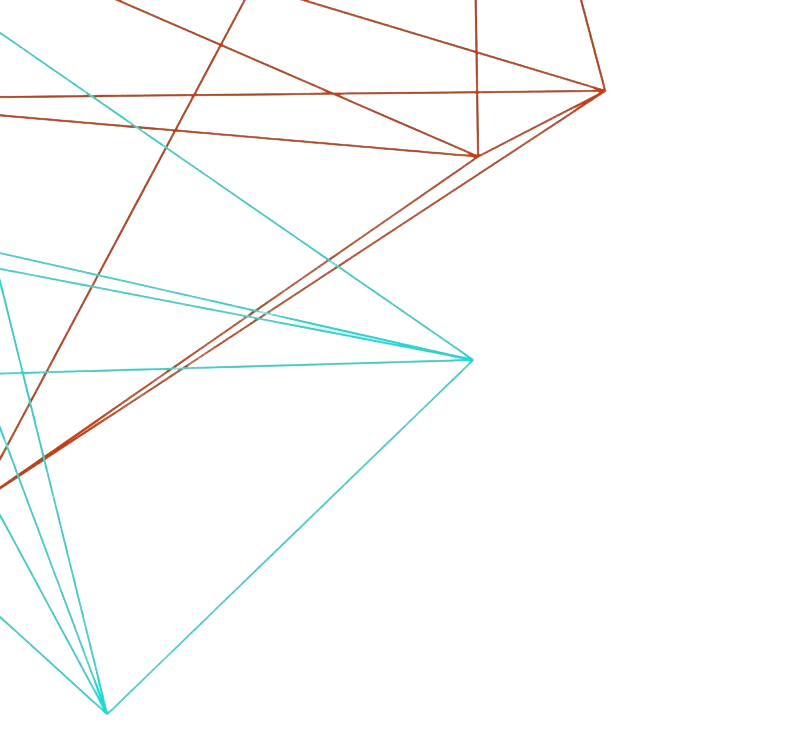
\includegraphics[angle=-90,origin=c,width=0.5\paperheight,height=0.5\paperwidth]{./logos/invert3.png}};
\tikz[remember picture,overlay] \node[opacity=0.3,inner sep=0pt, anchor=south east] at (current page.south east){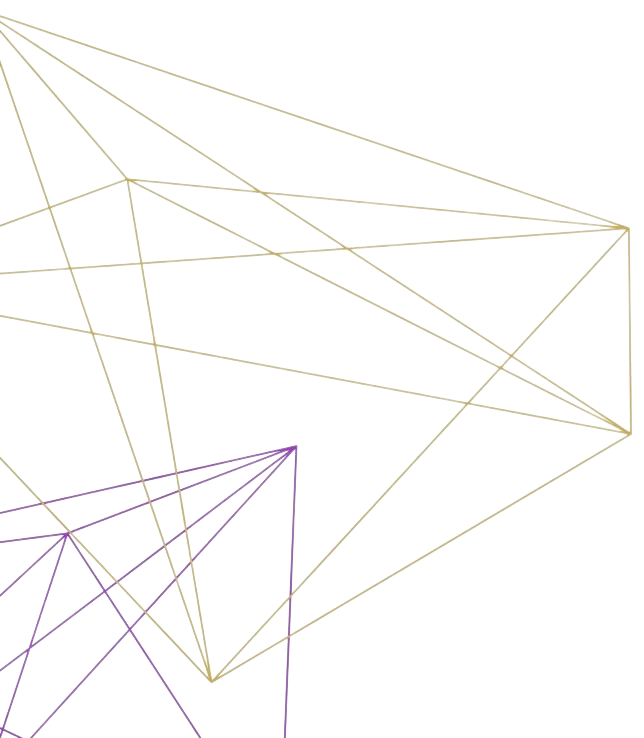
\includegraphics[angle=90,width=0.5\paperwidth,height=0.5\paperheight]{./logos/invert2.png}};

\thispagestyle{plain}
\newpage


\thispagestyle{fancy}
\tableofcontents


\newpage
\thispagestyle{plain}